\let\negmedspace\undefined
\let\negthickspace\undefined
\documentclass[journal]{IEEEtran}
\usepackage[a5paper, margin=10mm, onecolumn]{geometry}
%\usepackage{lmodern} % Ensure lmodern is loaded for pdflatex
\usepackage{tfrupee} % Include tfrupee package

\setlength{\headheight}{1cm} % Set the height of the header box
\setlength{\headsep}{0mm}     % Set the distance between the header box and the top of the text

\usepackage{gvv-book}
\usepackage{gvv}
\usepackage{cite}
\usepackage{amsmath,amssymb,amsfonts,amsthm}
\usepackage{algorithmic}
\usepackage{graphicx}
\usepackage{textcomp}
\usepackage{xcolor}
\usepackage{txfonts}
\usepackage{listings}
\usepackage{enumitem}
\usepackage{mathtools}
\usepackage{gensymb}
\usepackage{comment}
\usepackage[breaklinks=true]{hyperref}
\usepackage{tkz-euclide} 
\usepackage{listings}
% \usepackage{gvv}                                        
\def\inputGnumericTable{}                                 
\usepackage[latin1]{inputenc}                                
\usepackage{color}                                            
\usepackage{array}                                            
\usepackage{longtable}                                       
\usepackage{calc}                                             
\usepackage{multirow}                                         
\usepackage{hhline}                                           
\usepackage{ifthen}                                           
\usepackage{lscape}
\usepackage{pgfplots}
\begin{document}

\bibliographystyle{IEEEtran}
\vspace{3cm}

\title{1-1.5-32}
\author{AI24BTECH11033-Tanishq Rajiv Bhujbale}
% \maketitle
% \newpage
% \bigskip
{\let\newpage\relax\maketitle}

\renewcommand{\thefigure}{\theenumi}
\renewcommand{\thetable}{\theenumi}
\setlength{\intextsep}{10pt} % Space between text and floats


\numberwithin{equation}{enumi}
\numberwithin{figure}{enumi}
\renewcommand{\thetable}{\theenumi}


\textbf{Question}:\\
Find the ratio in which the line segment joining the points $\brak{1,-3}$ and $\brak{4, 5}$ is divided by $X$ axis.

\textbf{Solution}:\\

\begin{tikzpicture}
    \begin{axis}[
        axis lines = middle,
        xlabel = $x$,
        ylabel = $y$,
        xmin = 0, xmax = 5,
        ymin = -4, ymax = 6,
        grid = both,
        width=10cm, height=10cm,
        xtick={0,1,...,5},
        ytick={-4,-3,...,6},
        major grid style={line width=.2pt,draw=gray!30},
        minor grid style={line width=.1pt,draw=gray!10},
        every axis label/.append style={font=\small},
        every axis title/.append style={font=\small},
        every node near coord/.append style={font=\small}
    ]
    
    % Coordinates of A and B
    \addplot[only marks, red, mark=*, mark options={scale=1.5}] coordinates {(1,-3) (4,5)};
    \node[label={below right:{$A(1,-3)$}},circle,fill,inner sep=1.5pt] at (axis cs:1,-3) {};
    \node[label={above right:{$B(4,5)$}},circle,fill,inner sep=1.5pt] at (axis cs:4,5) {};
    
    % Line segment AB
    \addplot[domain=1:4,blue,thick] {2.6667*x - 5.6667};
    
    % Correct Point P (intersection with X-axis)
    \addplot[only marks, red, mark=*, mark options={scale=1.5}] coordinates {(2.125,0)};
    \node[label={above left:{$P(2.125,0)$}},circle,fill,inner sep=1.5pt] at (axis cs:2.125,0) {};
    
    % Ratio
    \node at (axis cs:2.5, 2) [green, font=\small] {Ratio $3:5$};
    
    \end{axis}
\end{tikzpicture}

1. \textbf{Equation of the Line Segment:}
The line segment joining $A=\brak{1,-3}$ and $B=\brak{4,5}$ can be expressed parametrically as:

   $$\frac{x-x_1}{x_2-x_1}=\frac{y-y_1}{y_2-y_1}$$

   where $(x_1,y_1)=(1,-3)$ and $(x_2,y_2)=(4,5)$.

   So,

   $$\frac{x-1}{4-1}=\frac{y+3}{5+3}$$

   Simplify to:

   $$\frac{x-1}{3}=\frac{y+3}{8}$$

2. \textbf{Finding Intersection with the \( x \)-Axis:}

   The intersection with the $x$-axis occurs when $y=0$. Substitute $y=0$ into the parametric equation:

   $$\frac{x-1}{3}=\frac{0+3}{8}$$

   Simplify:

   $$\frac{x-1}{3}=\frac{3}{8}$$

   Solving for $x$:

   $$x-1=\frac{3 \cdot 3}{8}=\frac{9}{8}$$

   $$x=1+\frac{9}{8}=\frac{8+9}{8}=\frac{17}{8}$$

   Therefore, the point of intersection with the $x$-axis is $\brak{\frac{17}{8}, 0}$.

3. \textbf{Using Section Formula to Find Ratio:}

   Let this point $\brak{\frac{17}{8},0}$ divide the segment $AB$ in the ratio $k:1$. The section formula for a point dividing a line segment in the ratio $k:1$ is given by:

   $$\brak{\frac{kx_2+x_1}{k+1},\frac{ky_2+y_1}{k+1}}$$

   Here, substituting the coordinates $A=(1,-3)$ and $B=(4,5)$:

   $$\brak{\frac{k \cdot 4+1}{k+1},\frac{k \cdot 5-3}{k+1}}=\brak{\frac{17}{8},0}$$

   Equate the $y$-coordinates:

   $$\frac{k \cdot 5-3}{k+1}=0$$

   $$k \cdot 5-3=0$$

   $$k=\frac{3}{5}$$

   Now, we need to verify the $x$-coordinate:

   $$\frac{\frac{3}{5} \cdot 4 + 1}{\frac{3}{5} + 1} = \frac{\frac{12}{5} + 1}{\frac{8}{5}} = \frac{\frac{12 + 5}{5}}{\frac{8}{5}} = \frac{\frac{17}{5}}{\frac{8}{5}} = \frac{17}{8}$$

   This confirms that our ratio $k=\frac{3}{5}$ is correct.

   Hence, the ratio in which the line segment joining the points $(1,-3)$ and $(4,5)$ is divided by the $x$-axis is $3:5$.

   $$\text{Ratio}=\frac{3}{5}:1=3:5$$
\end{document}

